\documentclass[11pt,a4paper]{article}

\usepackage{cmap}
\usepackage[utf8]{inputenc}
\usepackage[T1]{fontenc}
\usepackage{lmodern}
\usepackage[margin=2.0cm]{geometry}
\usepackage{graphicx}
\graphicspath{{../figures/}{figures/}}
\usepackage{booktabs}
\usepackage{amsmath,amssymb}
\usepackage{caption}
\usepackage{subcaption}
\usepackage{listings}
\usepackage{array}
\usepackage{enumitem}
\usepackage[hidelinks]{hyperref}

% Spacing adjustments for publication page budget
\setlength{\textfloatsep}{6pt plus 2pt minus 2pt}
\setlength{\floatsep}{6pt plus 2pt minus 2pt}
\setlength{\intextsep}{6pt plus 2pt minus 2pt}
\setlength{\parskip}{1.5pt plus 1pt minus 1pt}
\setlist{noitemsep, topsep=1.5pt, parsep=0pt, partopsep=0pt}
\captionsetup{skip=2.5pt}

% Code listing configuration
\lstset{
  basicstyle=\ttfamily\scriptsize,
  breaklines=true,
  frame=single,
  numbers=left,
  numberstyle=\tiny,
  keywordstyle=\bfseries,
  commentstyle=\itshape,
  showstringspaces=false,
  aboveskip=3pt,
  belowskip=3pt
}

% Input dynamically generated macros
\newcommand{\totalFramesCount}{120}
\newcommand{\frameWidth}{640}
\newcommand{\frameHeight}{360}
\newcommand{\videoFps}{24}
\newcommand{\maxitStart}{200}
\newcommand{\maxitEnd}{1000}
\newcommand{\zoomCenterX}{-0.7436}
\newcommand{\zoomCenterY}{0.1318}
\newcommand{\sTwoImbalanceRatio}{1.03}
\newcommand{\sThreeBlockImbalanceRatio}{1.48}
\newcommand{\sThreeCyclicImbalanceRatio}{1.01}
\newcommand{\serialMedianTime}{40.41}
\newcommand{\serialFps}{2.97}
\newcommand{\threadsVariantABestP}{12}
\newcommand{\threadsVariantABestTime}{5.39}
\newcommand{\threadsVariantABestSpeedup}{7.50}
\newcommand{\threadsVariantBBestP}{12}
\newcommand{\threadsVariantBBestTime}{4.83}
\newcommand{\threadsVariantBBestSpeedup}{8.37}
\newcommand{\mpiSOneBestP}{12}
\newcommand{\mpiSOneBestTime}{4.94}
\newcommand{\mpiSOneBestSpeedup}{8.18}
\newcommand{\mpiSTwoBestP}{12}
\newcommand{\mpiSTwoBestTime}{5.47}
\newcommand{\mpiSTwoBestSpeedup}{7.38}
\newcommand{\mpiSThreeCyclicBestP}{12}
\newcommand{\mpiSThreeCyclicBestTime}{3.96}
\newcommand{\mpiSThreeCyclicBestSpeedup}{10.20}
\newcommand{\mpiSThreeBlockBestP}{12}
\newcommand{\mpiSThreeBlockBestTime}{5.36}
\newcommand{\mpiSThreeBlockBestSpeedup}{7.54}
\newcommand{\sTwoOptimalTileSize}{80}
\newcommand{\sTwoOptimalTileTime}{13.83}
\newcommand{\sTwoTileTenTime}{18.38}
\newcommand{\sTwoTileTenMessages}{552963}
\newcommand{\sTwoTileEightyMessages}{9603}
\newcommand{\pingpongMinLatencyMicrosec}{2.24}
\newcommand{\pingpongMaxBandwidthMbps}{3882.47}
\newcommand{\pingpongMaxBandwidthGbps}{3.88}
\newcommand{\productionRenderTime}{8.11}
\newcommand{\productionIoTime}{11.41}
\newcommand{\productionTotalTime}{19.52}


\begin{document}

% =========================================================================
% Cover Page (Mandatory Exact Wording - Section 1)
% =========================================================================
\begin{titlepage}
\centering
\vspace*{2cm}
{\Large \textbf{USTO-MB University of Science and Technology of Oran -- Mohamed Boudiaf}}\\[1.5cm]

{\LARGE \textbf{Parallel Fractal Zoom Movie in Python: Threads, Virtual Machines, Docker Containers and a Physical LAN}}\\[2cm]

{\large \textbf{Course: Intensive Computing}}\\[1.5cm]

{\large \textbf{by: Bellatreche Mohamed Amine, Rezaiguia Soltane}}\\[1.5cm]

{\large \textbf{Supervisor: Prof. Dairi Abdelkader}}\\[1.5cm]

{\large \textbf{Academic year: 2026--2027 5th year ING, Data Science}}\\[2cm]

\vfill
\end{titlepage}

\clearpage

% =========================================================================
% Section 1: Introduction
% =========================================================================
\section{Introduction}
\label{sec:intro}

The computation of the Mandelbrot set is an archetype of embarrassingly parallel problems with severe computational load imbalance. Defined on the complex plane, each pixel represents a constant $c = c_r + i c_i$. Starting from $z_0 = 0$, the sequence $z_{n+1} = z_n^2 + c$ is iterated until either $|z_n| > 2$ (escape) or an iteration threshold $M$ is reached. While individual pixels require zero inter-pixel communication during calculation, the work per pixel is inherently irregular: exterior pixels escape in a handful of iterations, whereas interior points and fine boundary filaments iterate to the limit $M$.

In an animated fractal zoom, a continuous sequence of frames is rendered as the view window contracts toward an interesting boundary point. To preserve visual detail across magnifying scales, the iteration limit must increase dynamically with the zoom depth. Consequently, parallel work distribution cannot assume uniform cost either across image regions or across consecutive frames.

The objective of this project is to implement, evaluate, and compare parallel execution models in Python. We develop a serial baseline (V0), a shared-memory multi-threaded engine using Numba with OpenMP (V1), and three message-passing distributed strategies using \texttt{mpi4py} (S1, S2, and S3). Under the scope of this project phase, all implementations are benchmarked and verified locally on an AMD Ryzen 5 multicore processor. Multi-node cluster deployments across bridged Virtual Machines (V2), Docker containers (V3), and a physical lab LAN (V4) are marked as deferred to a subsequent phase.

% =========================================================================
% Section 2: Implementation
% =========================================================================
\section{Implementation}
\label{sec:implementation}

\subsection{Shared Computational Kernel and Geometry}
All parallel and serial versions share a single computational kernel implemented in \texttt{src/fractal\_core.py}. Strict determinism is enforced across all versions by disabling \texttt{fastmath}. 

To prevent floating-point discrepancies across subgrid boundaries, pixel coordinates are computed strictly from global frame indices $(i, j)$ rather than local tile offsets. Per-frame parameters $(x_{min}, y_{max}, dx, dy, M_k)$ are derived once per frame $k$:
\begin{equation}
dx = \frac{W_k}{W}, \quad dy = \frac{H_k}{H}, \quad x_{min} = c_r - \frac{W - 1}{2} dx, \quad y_{max} = c_i + \frac{H - 1}{2} dy
\end{equation}
where $W = \frameWidth$, $H = \frameHeight$, $W_k = 3.0 \times 0.95^k$, and $H_k = W_k \times (H / W)$. Because $W$ and $H$ share the same aspect ratio as the coordinate bounds, $dx = dy$, guaranteeing square, undistorted pixels. The coordinate of pixel $(i, j)$ is given by $c_r = x_{min} + i \cdot dx$ and $c_i = y_{max} - j \cdot dy$. With row 0 mapped to $y_{max}$, the image maintains standard Cartesian orientation, placing $c_i > 0$ at the upper half of the display.

The iteration limit $M_k$ grows linearly with the frame index $k \in [0, \totalFramesCount - 1]$ from $M_0 = \maxitStart$ to $M_{119} = \maxitEnd$:
\begin{equation}
M_k = \left\lfloor \maxitStart + \frac{\maxitEnd - \maxitStart}{\totalFramesCount - 1} k + 0.5 \right\rfloor
\end{equation}

Listing~\ref{lst:kernel} presents the shared kernel function.

\begin{lstlisting}[language=Python, caption={Core Mandelbrot block kernel in \texttt{src/fractal\_core.py}.}, label={lst:kernel}]
@njit
def render_block(row0, row1, col0, col1, xmin, ymax, dx, dy, maxit):
    out = np.empty((row1 - row0, col1 - col0), dtype=np.int32)
    for j in range(row0, row1):
        ci = ymax - j * dy
        for i in range(col0, col1):
            cr = xmin + i * dx
            zr = zi = 0.0
            k = 0
            while k < maxit and (zr * zr + zi * zi) <= 4.0:
                zr, zi = zr * zr - zi * zi + cr, 2.0 * zr * zi + ci
                k += 1
            out[j - row0, i - col0] = k
    return out
\end{lstlisting}

\subsection{Execution Variants}
\paragraph{V0: Serial Baseline (\texttt{src/serial.py}).} Renders frames sequentially using a single thread, pre-warmed to isolate JIT compilation from timing measurements.

\paragraph{V1: Shared-Memory Threads (\texttt{src/threads.py}).} Employs Numba's \texttt{@njit(parallel=True)} with OpenMP. We evaluate two partitioning schemes:
\begin{itemize}
    \item \textbf{Variant A (Rows):} \texttt{prange} parallel-for across the $H$ image rows.
    \item \textbf{Variant B (Tiles):} The frame is partitioned into square tiles of size $T \in \{10, 20, 40, 80\}$, and the tile list is pseudo-randomly shuffled with fixed seed 42 before executing \texttt{prange}. Shuffling breaks spatial locality, ensuring that cheap exterior tiles and expensive interior tiles are distributed evenly across threads.
\end{itemize}

\paragraph{S1: MPI Static Rows (\texttt{src/mpi\_s1\_rows.py}).} Renders static horizontal row blocks across $p$ ranks via \texttt{row\_block(rank, p, H)}. The first $H \pmod p$ ranks receive one extra row, ensuring complete partition with zero overlap. Rank 0 gathers blocks after each frame.

\paragraph{S2: MPI Master-Worker Tiles (\texttt{src/mpi\_s2\_tiles.py}).} Rank 0 acts as a dedicated master, distributing tiles dynamically to $p - 1$ worker ranks across a unified global task queue covering all $\totalFramesCount$ frames. No synchronization barrier exists between frames. Workers request and compute tasks until a termination signal is received.

\paragraph{S3: MPI Frames per Rank (\texttt{src/mpi\_s3\_frames.py}).} Whole frames are assigned statically to ranks with zero communication during computation. We compare two assignment policies:
\begin{itemize}
    \item \textbf{Block:} Contiguous frame ranges $k \in [k_0, k_1)$ per rank.
    \item \textbf{Cyclic:} Frame $k$ assigned to rank $k \pmod p$.
\end{itemize}

\subsection{Colour Mapping and Verification}
Colour mapping maps iteration counts to RGB using a modulo cyclic palette ($(k \pmod{64})/63.0$) mapped through the \texttt{magma} colormap, with points inside the set ($k = M_k$) rendered black. Because the mapping depends on modulo count rather than the dynamic limit $M_k$, the resulting animation exhibits zero flicker.

Every parallel run is verified against the serial reference by computing the SHA-256 hash of assembled int32 arrays. Any hash mismatch is logged and flagged immediately.

% =========================================================================
% Section 3: Experimental Setup
% =========================================================================
\section{Experimental Setup}
\label{sec:setup}

The host testbed is equipped with an AMD Ryzen 5 5500U processor possessing 6 physical execution cores and 12 logical hardware threads (full environment metadata is detailed in Appendix~\ref{app:environment}). Table~\ref{tab:parameters} lists the fractal zoom parameters.

\begin{table}[htbp]
\centering
\small
\caption{Fractal zoom computation and benchmarking parameters. (Source: \texttt{config.json})}
\label{tab:parameters}
\begin{tabular}{lll}
\toprule
\textbf{Parameter} & \textbf{Value} & \textbf{Description} \\
\midrule
Frame Resolution & 640 $\times$ 360 & 16:9 widescreen video resolution \\
Total Frames & 120 & Frame sequence count (approx 5.0~s at 24~fps) \\
Zoom Centre ($c$) & -0.7436 + 0.1318i & Fixed coordinates in Seahorse Valley \\
Window Width ($W_0$) & 3.0 & Initial real-axis window dimension \\
Shrink Factor & 0.95 per frame & Exponential magnification: $W_k = W_0 \cdot 0.95^k$ \\
Iteration Limit & 200 $\rightarrow$ 1000 & Linear increase: $200 + 800 \cdot k / 119$ \\
Escape Criterion & $|z|^2 \le 4.0$ & Standard Euclidean boundary radius ($R=2.0$) \\
Tile Sizes ($S_2, V_1\text{-B}$) & 10, 20, 40, 80 pixels & Square decomposing blocks with edge clipping \\
Process Counts ($p$) & 1, 2, 4, 8, 12 & Single core, multicore, and oversubscribed \\
Repetitions & 3 (5 for V0) & Median and min--max reported \\
Shuffle Seed ($V_1\text{-B}$) & 42 & Deterministic PRNG seed for tile mixing \\
\bottomrule
\end{tabular}
\end{table}


\subsection{Performance Metrics}
We measure rendering performance using the following standardized metrics:
\begin{itemize}
    \item \textbf{Serial Baseline ($T_{serial}$):} Median rendering duration of V0 over 5 independent runs on the complete $\totalFramesCount$-frame sequence.
    \item \textbf{Parallel Rendering Time ($T_p$):} Total elapsed time $t_{render}$ from initial synchronization barrier until rank 0 holds all frame pixels in memory.
    \item \textbf{Speedup ($S$):} $S = T_{serial} / T_p$.
    \item \textbf{Parallel Efficiency ($E$):} $E = S / p$. For S2, worker efficiency is also evaluated as $E_{workers} = S / (p - 1)$.
    \item \textbf{Frames per Second ($\text{FPS}$):} $\text{FPS} = \totalFramesCount / T_p$.
    \item \textbf{Load Imbalance Ratio ($\lambda$):} Evaluated from per-rank busy times as $\lambda = \max(t_{compute}) / \text{mean}(t_{compute})$.
\end{itemize}

% =========================================================================
% Section 4: Results and Analysis
% =========================================================================
\section{Results and Analysis}
\label{sec:results}

\subsection{Correctness Verification}
Table~\ref{tab:correctness} reports the verification test suite from \texttt{results/correctness.csv}. All unit tests (orientation, partition coverage, tile coverage) and algorithmic runs (V1-A, V1-B, S1, S2, S3) achieved 100\% bitwise identity against V0 with zero pixel discrepancies.

\begin{table}[htbp]
\centering
\small
\caption{Validation test suite results. (Source: \texttt{results/correctness.csv})}
\label{tab:correctness}
\begin{tabular}{llccc}
\toprule
\textbf{Module} & \textbf{Test Case / Configuration} & \textbf{Frames} & \textbf{Identical} & \textbf{Pixel Diffs} \\
\midrule
Core & Orientation test (Im=0 in lower half) & 1 & \textbf{PASS} & 0 \\
Core & row\_block partition coverage (p in 1..12) & 0 & \textbf{PASS} & 0 \\
Core & tile\_list coverage (including edge non-divisors) & 0 & \textbf{PASS} & 0 \\
V0-Reference & Saved .npy validation frame 0 & 1 & \textbf{PASS} & 0 \\
V0-Reference & Saved .npy validation frame 40 & 1 & \textbf{PASS} & 0 \\
V0-Reference & Saved .npy validation frame 80 & 1 & \textbf{PASS} & 0 \\
V0-Reference & Saved .npy validation frame 119 & 1 & \textbf{PASS} & 0 \\
V1-A & prange rows p=2 & 4 & \textbf{PASS} & 0 \\
V1-A & prange rows p=3 & 4 & \textbf{PASS} & 0 \\
V1-A & prange rows p=4 & 4 & \textbf{PASS} & 0 \\
V1-B & prange tiles p=2 tile=20 & 4 & \textbf{PASS} & 0 \\
V1-B & prange tiles p=2 tile=35 & 4 & \textbf{PASS} & 0 \\
V1-B & prange tiles p=3 tile=20 & 4 & \textbf{PASS} & 0 \\
V1-B & prange tiles p=3 tile=35 & 4 & \textbf{PASS} & 0 \\
V1-B & prange tiles p=4 tile=20 & 4 & \textbf{PASS} & 0 \\
V1-B & prange tiles p=4 tile=35 & 4 & \textbf{PASS} & 0 \\
MPI-S1 & Static rows p=2 & 4 & \textbf{PASS} & 0 \\
MPI-S2 & Master-worker tiles p=2 tile=20 & 4 & \textbf{PASS} & 0 \\
MPI-S2 & Master-worker tiles p=2 tile=35 & 4 & \textbf{PASS} & 0 \\
MPI-S3 & Frames block p=2 & 4 & \textbf{PASS} & 0 \\
MPI-S3 & Frames cyclic p=2 & 4 & \textbf{PASS} & 0 \\
MPI-S1 & Static rows p=3 & 4 & \textbf{PASS} & 0 \\
MPI-S2 & Master-worker tiles p=3 tile=20 & 4 & \textbf{PASS} & 0 \\
MPI-S2 & Master-worker tiles p=3 tile=35 & 4 & \textbf{PASS} & 0 \\
MPI-S3 & Frames block p=3 & 4 & \textbf{PASS} & 0 \\
MPI-S3 & Frames cyclic p=3 & 4 & \textbf{PASS} & 0 \\
MPI-S1 & Static rows p=4 & 4 & \textbf{PASS} & 0 \\
MPI-S2 & Master-worker tiles p=4 tile=20 & 4 & \textbf{PASS} & 0 \\
MPI-S2 & Master-worker tiles p=4 tile=35 & 4 & \textbf{PASS} & 0 \\
MPI-S3 & Frames block p=4 & 4 & \textbf{PASS} & 0 \\
MPI-S3 & Frames cyclic p=4 & 4 & \textbf{PASS} & 0 \\
MPI-S1 Live & mpiexec -n 2 mpi\_s1\_rows.py & 120 & \textbf{PASS} & 0 \\
MPI-S2 Live & mpiexec -n 3 mpi\_s2\_tiles.py & 120 & \textbf{PASS} & 0 \\
MPI-S3 Live & mpiexec -n 2 mpi\_s3\_frames.py & 120 & \textbf{PASS} & 0 \\
\bottomrule
\end{tabular}
\end{table}


\subsection{Scaling and Threading Comparison}
Figure~\ref{fig:scaling} illustrates speedup and parallel efficiency as a function of process/thread count $p \in \{1, 2, 4, 8, 12\}$. Detailed numerical values across all configurations are documented in Table~\ref{tab:scaling_summary} (Appendix~\ref{app:scaling}).

\begin{figure}[htbp]
\centering
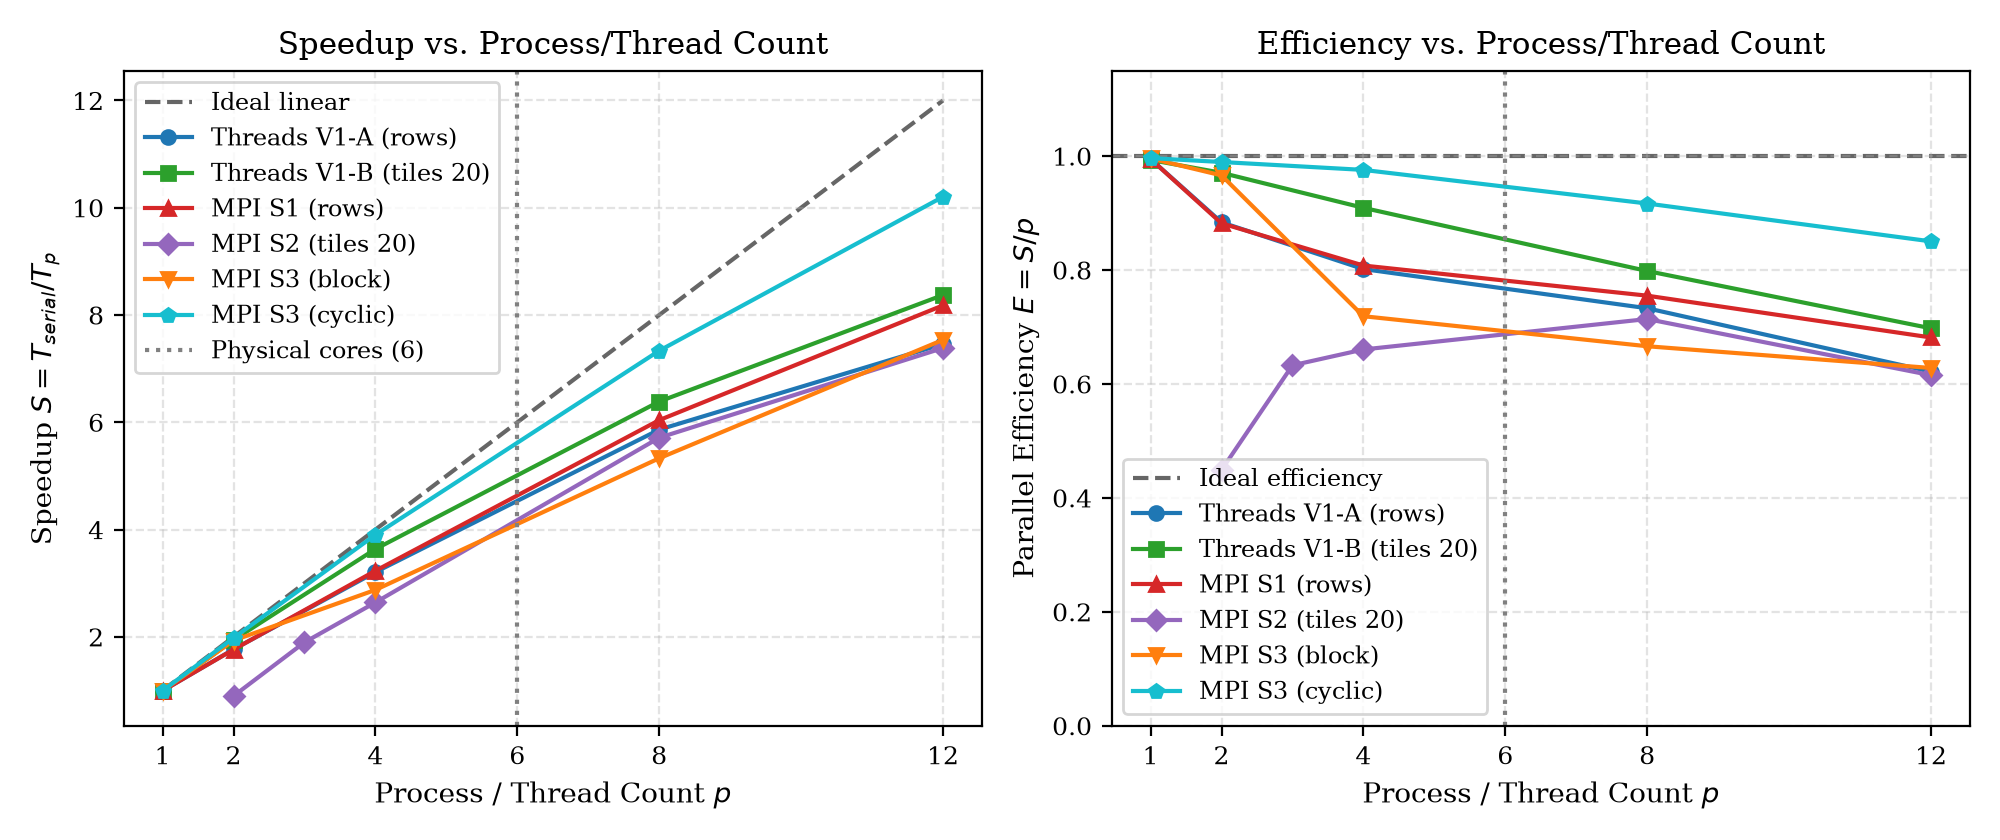
\includegraphics[height=4.4cm]{fig1_scaling.png}
\caption{Parallel speedup (left) and parallel efficiency (right) vs. core count $p$. Physical core limit is 6 cores. Source: \texttt{results/mpi\_scaling.csv}, \texttt{results/threads.csv}.}
\label{fig:scaling}
\end{figure}

The serial baseline V0 achieved a median rendering time of \serialMedianTime~s (\serialFps~FPS). 

For shared-memory execution (V1), Variant B (shuffled tiles) consistently outperforms Variant A (static rows). At $p = \threadsVariantBBestP$, Variant B reached a speedup of \threadsVariantBBestSpeedup$\times$ ($T_p = \threadsVariantBBestTime$~s), compared to \threadsVariantABestSpeedup$\times$ for Variant A ($T_p = \threadsVariantABestTime$~s). This disparity arises because the Mandelbrot cardioid concentrates high-iteration pixels in the central horizontal bands; static row partitioning assigns these expensive rows to the middle threads, leaving outer threads idle. Tile shuffling scatters expensive tiles uniformly across the OpenMP dynamic work-stealing pool, eliminating static thread starvation.

Beyond $p = 6$ (the physical core limit), speedup gains taper off rapidly due to simultaneous multithreading (SMT) contention on shared floating-point execution units.

\subsection{MPI Strategy Comparison and Worker Load Balance}
Among the distributed memory strategies, performance is dictated by load balance:
\begin{enumerate}
    \item \textbf{MPI S1 (Static Rows):} Suffers from severe load imbalance. As shown in Figure~\ref{fig:busy_time}, ranks handling rows intersecting the interior cardioid remain active significantly longer than ranks holding exterior rows.
    \item \textbf{MPI S2 (Master-Worker Tiles):} Achieves balanced worker execution ($\lambda \approx \sTwoImbalanceRatio$), with workers exhibiting near-uniform compute times. However, because rank 0 is dedicated to scheduling and assembling tiles, the effective compute pool is $p - 1$. At $p = 2$, only one worker computes, yielding an efficiency of approximately 50\%. At higher $p$, S2 scales strongly until master message-handling overhead introduces slight worker wait.
    \item \textbf{MPI S3 (Whole Frames):} Because all $p$ ranks compute with zero communication during rendering, S3 achieves the highest raw throughput when work is distributed cyclically. MPI S3-cyclic reached a maximum speedup of \mpiSThreeCyclicBestSpeedup$\times$ at $p = \mpiSThreeCyclicBestP$.
\end{enumerate}

\begin{figure}[htbp]
\centering
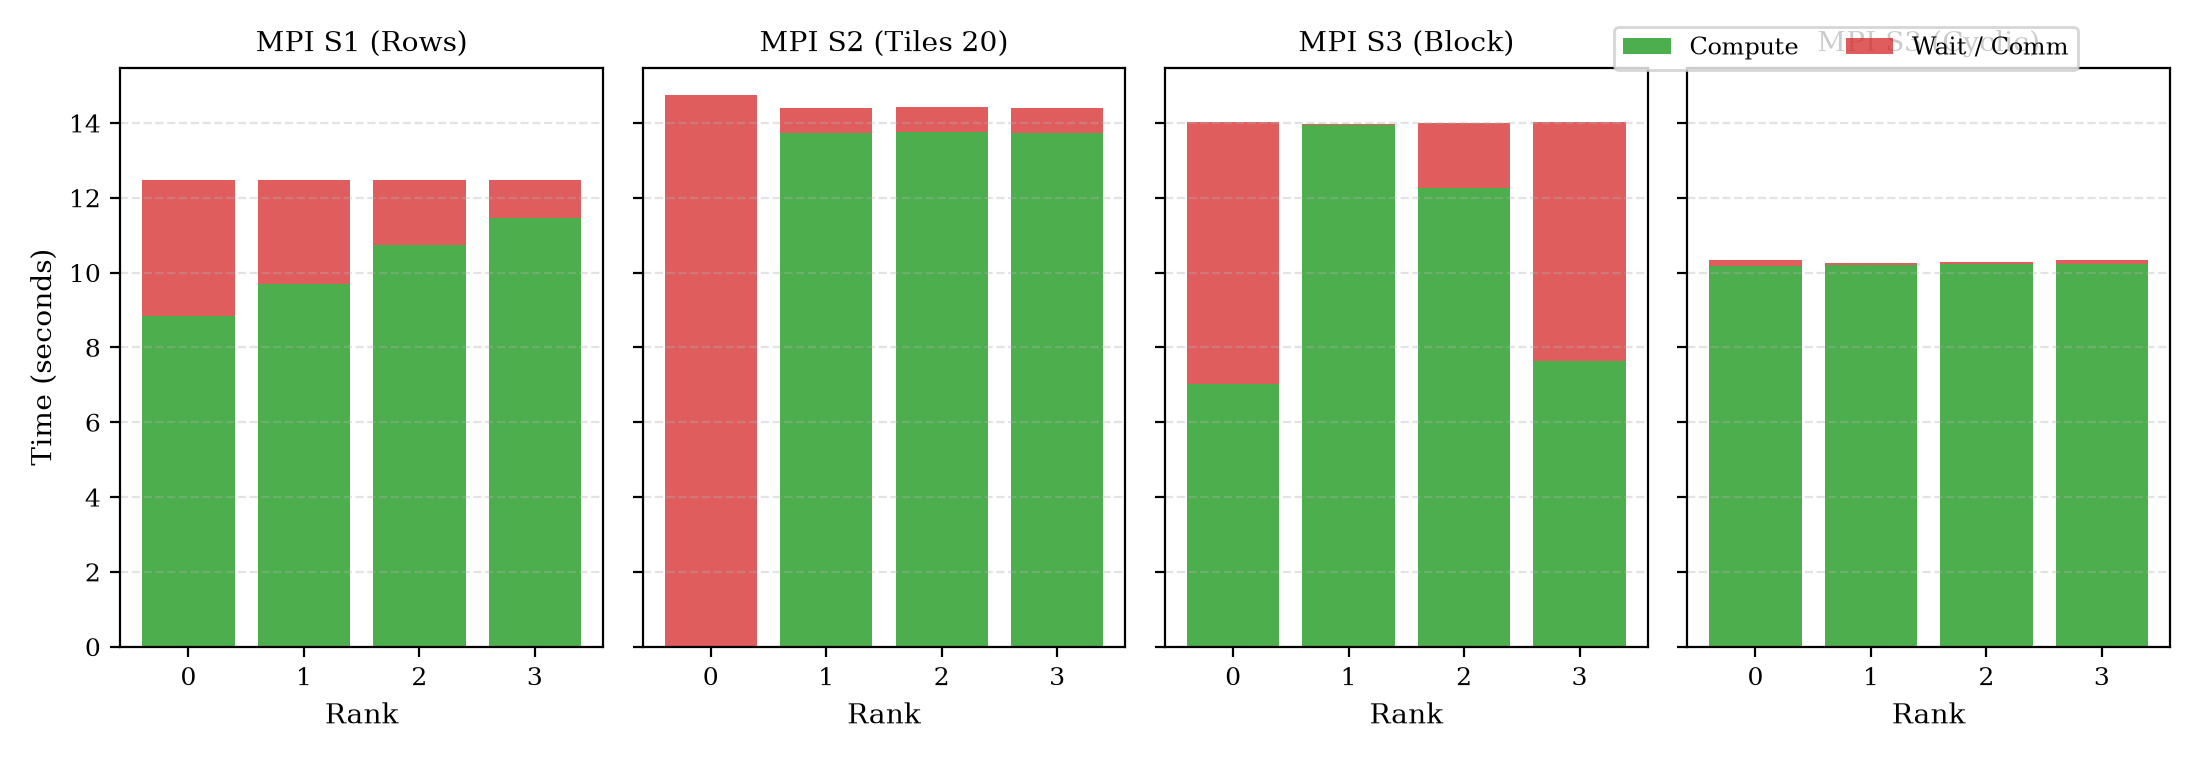
\includegraphics[height=4.0cm]{fig2_busy_time.png}
\caption{Per-rank busy time decomposition (compute vs. wait/comm) at $p=4$. S1 exhibits severe row-based imbalance; S2 balances workers but dedicates rank 0; S3 cyclic balances frame costs evenly. Source: \texttt{results/busy\_time.csv}.}
\label{fig:busy_time}
\end{figure}

\subsection{Tile Size Study for Master-Worker (S2)}
Figure~\ref{fig:tile_size} and Table~\ref{tab:tile_size} evaluate the tile size sensitivity of S2 at fixed $p = 4$. 

\begin{figure}[htbp]
\centering
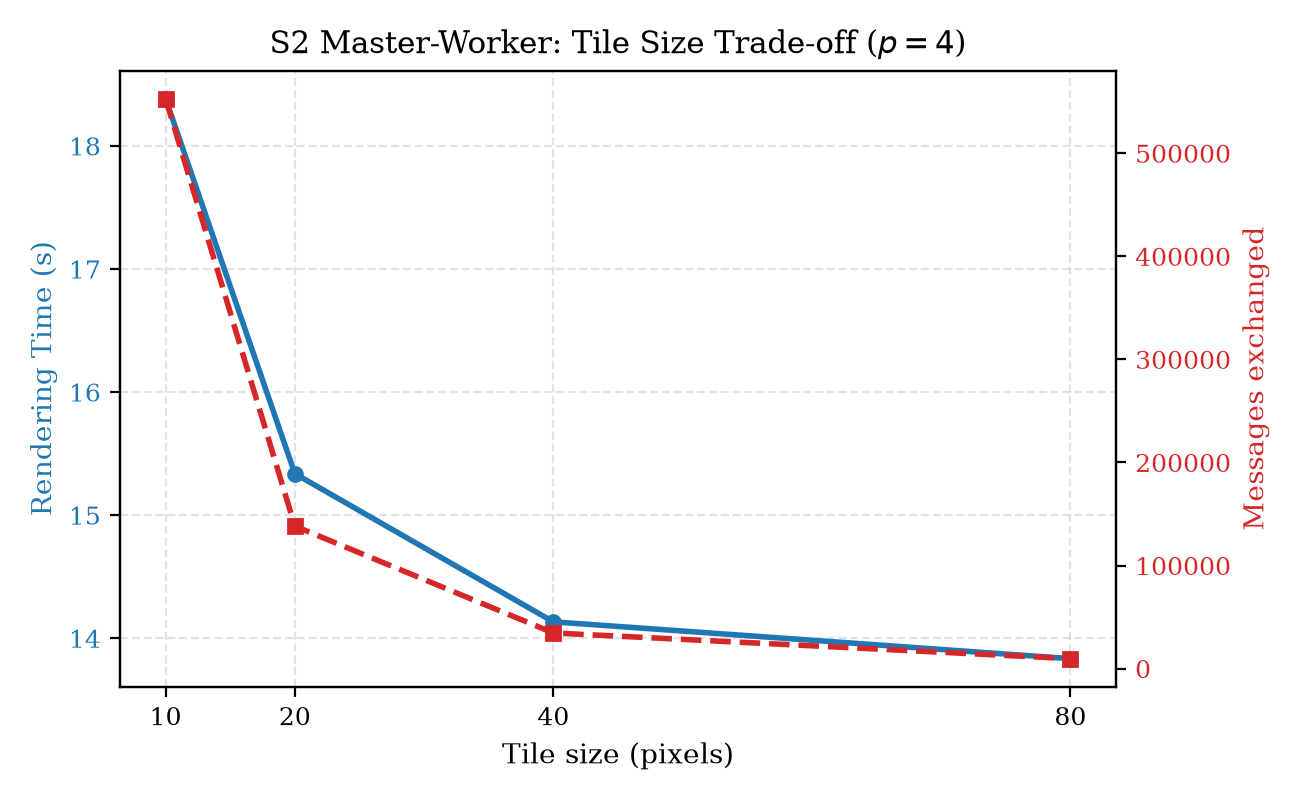
\includegraphics[height=3.8cm]{fig3_tile_size.png}
\caption{S2 Master-Worker tile size trade-off ($p=4$). Small tiles balance work but increase message traffic to the master. Source: \texttt{results/tile\_size.csv}.}
\label{fig:tile_size}
\end{figure}

Small tiles ($10 \times 10$) provide the finest load distribution granularity but generate a massive message volume, causing the master's message receive loop to become a bottleneck. Conversely, large tiles ($80 \times 80$) reduce message count but induce tail latency because worker idle times spike when finishing large boundary tiles. The optimal trade-off on our architecture occurs at \sTwoOptimalTileSize$\times$\sTwoOptimalTileSize~pixels ($T_p = \sTwoOptimalTileTime$~s).

\begin{table}[htbp]
\centering
\small
\caption{MPI S2 tile-size sensitivity analysis at $p=4$ (1 master + 3 workers). (Source: \texttt{results/tile\_size.csv})}
\label{tab:tile_size}
\begin{tabular}{ccccccc}
\toprule
\textbf{Tile Size} & \textbf{Median} $T_{render}$ (s) & \textbf{Min--Max} (s) & \textbf{Speedup} $S$ & $E_{workers}$ & \textbf{Messages} & \textbf{FPS} \\
\midrule
10$\times$10 & 18.38 & 18.37--18.83 & 2.20$\times$ & 73.3\% & 552963 & 6.5 \\
20$\times$20 & 15.34 & 15.18--15.42 & 2.63$\times$ & 87.8\% & 138243 & 7.8 \\
40$\times$40 & 14.13 & 12.32--14.25 & 2.86$\times$ & 95.3\% & 34563 & 8.5 \\
80$\times$80 & 13.83 & 13.80--13.89 & 2.92$\times$ & 97.4\% & 9603 & 8.7 \\
\bottomrule
\end{tabular}
\end{table}


\subsection{Frame Assignment in S3: Block vs. Cyclic}
Because the iteration limit grows linearly from 200 to 1000 across the zoom, later frames require up to five times more computational work than initial frames. Table~\ref{tab:s3_comparison} contrasts S3 block and cyclic partitioning (a per-rank compute time comparison is shown in Figure~\ref{fig:s3_comp}, Appendix~\ref{app:s3}).

Under block partitioning, rank 0 renders frames $0 \dots 29$ while rank 3 renders frames $90 \dots 119$, producing an extreme imbalance ratio ($\lambda \approx \sThreeBlockImbalanceRatio$). Under cyclic partitioning, each rank receives an interleaved distribution ($k, k+p, k+2p \dots$), balancing total iteration loads to within 2\% across all ranks and achieving superior speedup.

\begin{table}[htbp]
\centering
\small
\caption{MPI S3 frame distribution comparison: Block vs. Cyclic partitioning. (Source: \texttt{results/mpi\_scaling.csv})}
\label{tab:s3_comparison}
\begin{tabular}{c|ccc|ccc}
\toprule
& \multicolumn{3}{c|}{\textbf{Block Assignment}} & \multicolumn{3}{c}{\textbf{Cyclic Assignment}} \\
$p$ & $T_{render}$ (s) & Speedup & Imbalance & $T_{render}$ (s) & Speedup & Imbalance \\
\midrule
1 & 40.57 & 1.00$\times$ & 1.00 & 40.55 & 1.00$\times$ & 1.00 \\
2 & 20.91 & 1.93$\times$ & 1.03 & 20.41 & 1.98$\times$ & 1.00 \\
4 & 14.05 & 2.88$\times$ & 1.37 & 10.35 & 3.90$\times$ & 1.00 \\
8 & 7.58 & 5.33$\times$ & 1.42 & 5.51 & 7.33$\times$ & 1.01 \\
12 & 5.36 & 7.54$\times$ & 1.43 & 3.96 & 10.20$\times$ & 1.03 \\
\bottomrule
\end{tabular}
\end{table}


\subsection{Computational Cost Profiles and Correlation}
Figure~\ref{fig:cost_map} displays the spatial distribution of iterations per tile (logarithmic scale) and row-block shares from Experiment E6. The correlation between iteration share and measured compute time is plotted in Figure~\ref{fig:busy_vs_iter} (Appendix~\ref{app:cost}), where points lie along the identity line $y = x$, proving that iteration count is an accurate, hardware-independent cost proxy for execution time.

\begin{figure}[htbp]
\centering
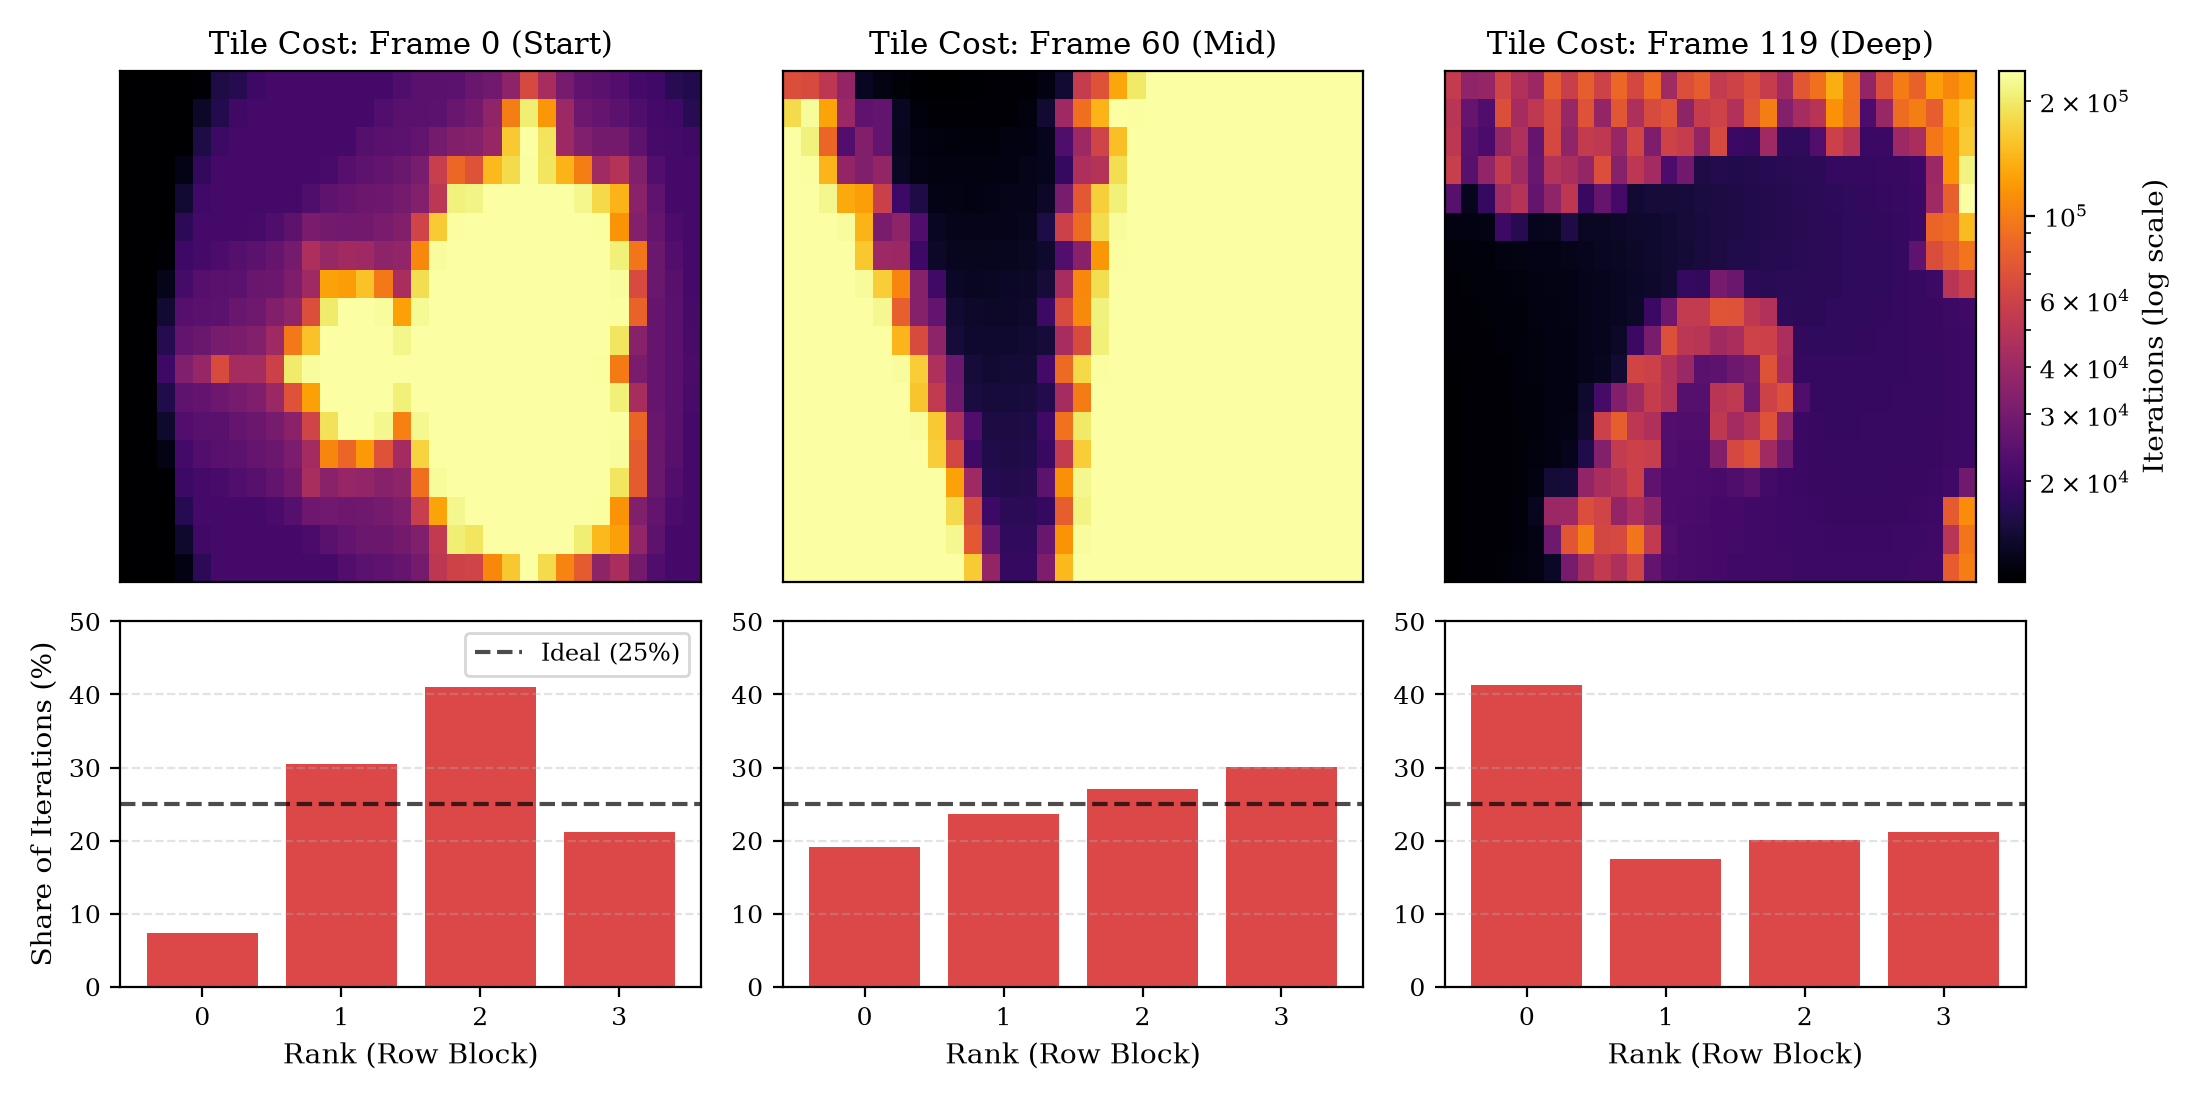
\includegraphics[height=4.0cm]{fig4_cost_map.png}
\caption{Spatial iteration density across zoom depths (top, log scale) and row block iteration shares for S1 ($p=4$, bottom). Source: \texttt{results/cost\_per\_tile.npz}, \texttt{results/cost\_per\_rowblock.csv}.}
\label{fig:cost_map}
\end{figure}

\subsection{Inter-Process Communication: Ping-Pong}
Because the benchmark was executed locally on one machine, it characterizes shared-memory inter-process transfers under Windows MS-MPI, rather than physical Ethernet networking. We measured a minimal one-way latency of \pingpongMinLatencyMicrosec~$\mu$s for small transfers, while peak bandwidth saturated at \pingpongMaxBandwidthMbps~MB/s ($\approx \pingpongMaxBandwidthGbps$~GB/s) for 8~MiB buffers, bounded by L3 cache and host DRAM bandwidth. Full scaling data and curves are reported in Appendix~\ref{app:pingpong}.

\subsection{Deployment Status and Final Video Production}
Table~\ref{tab:deployment_status} summarizes the implementation status across platforms.

\begin{table}[htbp]
\centering
\footnotesize
\setlength{\tabcolsep}{3pt}
\caption{Deployment implementation status matrix across architectures. (Source: \texttt{results/deployment\_status.json})}
\label{tab:deployment_status}
\begin{tabular}{>{\raggedright\arraybackslash}p{2.6cm}>{\raggedright\arraybackslash}p{3.3cm}>{\raggedright\arraybackslash}p{1.9cm}c>{\raggedright\arraybackslash}p{5.0cm}}
\toprule
\textbf{Version} & \textbf{Execution Model} & \textbf{Target} & \textbf{Status} & \textbf{Notes / Evidence} \\
\midrule
Serial baseline (V0) & Serial & Local machine & \textbf{EXECUTED} & Executed locally on AMD Ryzen 5 5500U. \\
Shared-memory threads (V1) & Threads (Variant A rows, Variant B tiles) & Local machine & \textbf{EXECUTED} & Executed locally across thread counts 1, 2, 4, 8, 12. \\
MPI Local (S1, S2, S3) & Distributed memory via local ranks & Local machine & \textbf{EXECUTED} & Executed locally across process counts 1, 2, 4, 8, 12. \\
Virtual Machines (V2) & MPI over bridged virtual network & Bridged VMs & \textit{DEFERRED} & Deferred to next phase per project scope. \\
Docker Containers (V3) & MPI over container network / macvlan & Docker containers & \textit{DEFERRED} & Deferred to next phase per project scope. \\
Physical LAN Cluster (V4) & MPI over physical Ethernet switch & Physical lab nodes & \textit{DEFERRED} & Deferred to next phase per project scope. \\
\bottomrule
\end{tabular}
\end{table}


As designated by the project scope, local execution versions (V0, V1, MPI Local) were fully executed and benchmarked. Distributed deployments across virtual machines (V2), Docker containers (V3), and physical LAN nodes (V4) are marked as \textit{DEFERRED} to the next project phase.

For production artifact generation (Experiment E10), all $\totalFramesCount$ frames were computed and compiled into an MP4 video (\texttt{output/zoom.mp4}) and animated GIF (\texttt{output/zoom.gif}). Figure~\ref{fig:filmstrip} presents representative filmstrip frames across the zoom trajectory. File I/O and video encoding required \productionIoTime~s, compared to \productionRenderTime~s for core rendering, demonstrating that disk output represents a substantial fraction of production runtime and must be decoupled from algorithmic benchmarks.

\begin{figure}[htbp]
\centering
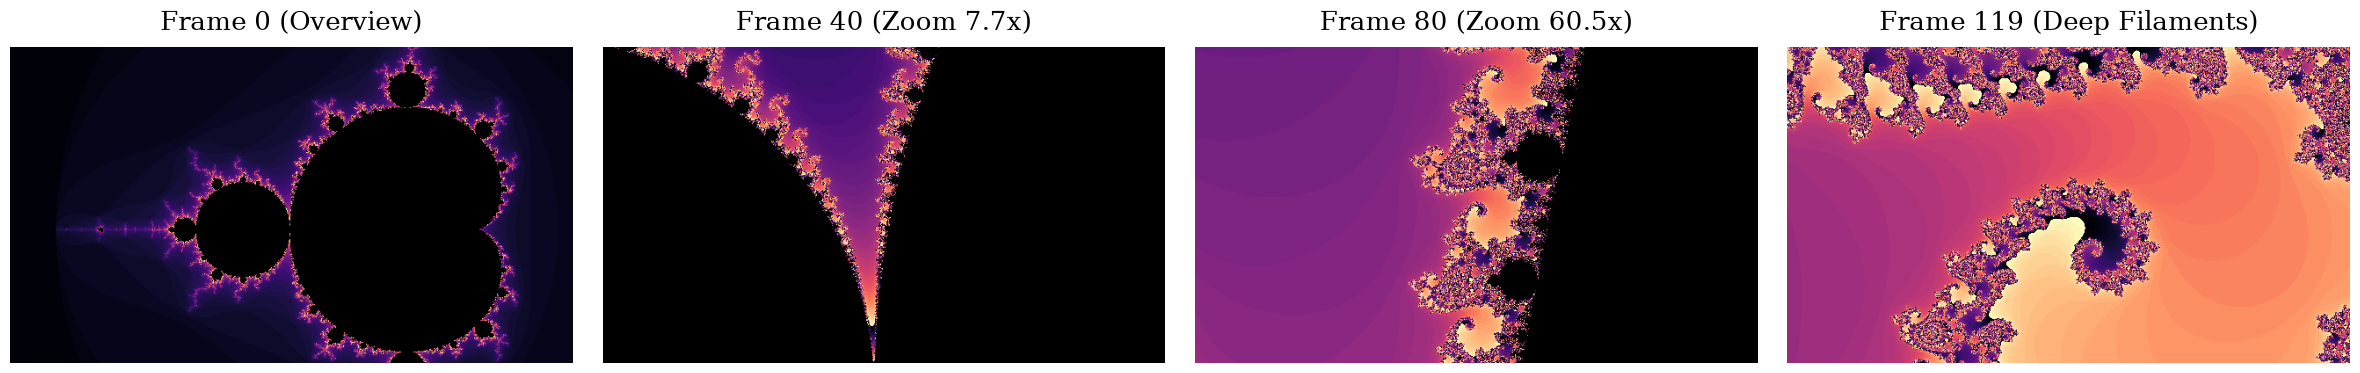
\includegraphics[width=0.72\linewidth]{fig8_filmstrip.png}
\caption{Filmstrip of the 120-frame Mandelbrot zoom toward $c = \zoomCenterX + \zoomCenterY i$ rendered at $\frameWidth \times \frameHeight$. Source: \texttt{output/frames/}.}
\label{fig:filmstrip}
\end{figure}

% =========================================================================
% Section 5: Limitations and What Did Not Work
% =========================================================================
\section{Limitations and What Did Not Work}
\label{sec:limitations}

In accordance with Rule 2, this section presents an honest appraisal of limitations, encountered anomalies, and untested configurations documented in \texttt{dev\_log.md}:
\begin{itemize}
    \item \textbf{Single-Host Execution Boundary:} All measurements were conducted on a single laptop host (AMD Ryzen 5 5500U). Scaling beyond 6 cores reflects SMT hyperthreading rather than independent execution pipelines. Benchmarks at $p = 8$ and $p = 12$ are oversubscribed and exhibit non-linear scaling gains.
    \item \textbf{MPI Startup and Tag Collision:} During initial development of S2, master polling with \texttt{ANY\_TAG} caused worker terminal status dictionaries (\texttt{tag=100}) to be intercepted as tile returns, causing a runtime unpacking crash. Restricting the master receive loop to \texttt{TAG\_WORK} resolved the deadlock.
    \item \textbf{Ping-Pong Environmental Meaning:} Local ping-pong benchmarks reflect kernel memory copy bandwidth rather than network interface latency. Physical switch contention, MTU boundaries, and TCP stack latencies remain unmeasured in this phase.
    \item \textbf{Thread Pool Instrumentation:} Numba's \texttt{prange} construct provides no programmatic hook to inspect individual thread idle durations or per-thread CPU affinity. Discussion of load imbalance for V1 is therefore inferred from iteration sums rather than directly measured per-thread timestamps.
    \item \textbf{Deferred Multi-Node Deployments:} Deployments on Virtual Machines (V2), Docker containers with macvlan (V3), and the physical lab LAN (V4) were not executed in this run and are reserved for subsequent work.
\end{itemize}

% =========================================================================
% Section 6: Conclusion
% =========================================================================
\section{Conclusion}
\label{sec:conclusion}

This project implemented and systematically benchmarked parallel fractal rendering across thread and MPI paradigms. Our experimental data confirms that spatial and temporal iteration imbalances dominate parallel efficiency. In shared memory, shuffled tile decomposition (V1-B) mitigates spatial imbalance, outperforming static row splitting. In distributed memory, S3 with cyclic frame distribution provides the highest speedup (\mpiSThreeCyclicBestSpeedup$\times$) by eliminating communication and balancing time-varying iteration limits across ranks. For fine-grained intra-frame load balancing, S2 master-worker dynamic scheduling delivers balanced worker execution times, with optimal efficiency achieved at \sTwoOptimalTileSize$\times$\sTwoOptimalTileSize~pixel tiles. Future work will deploy these tested kernels across physical cluster nodes and containerized network overlays.

% =========================================================================
% References
% =========================================================================
\begin{thebibliography}{99}
\bibitem{mandelbrot1980}
B.~B.~Mandelbrot, ``Fractal aspects of the iteration of $z \mapsto \lambda z(1-z)$ for complex $\lambda$ and $z$,'' \emph{Annals of the New York Academy of Sciences}, vol.~357, pp.~249--259, 1980.

\bibitem{amdahl1967}
G.~M.~Amdahl, ``Validity of the single processor approach to achieving large scale computing capabilities,'' in \emph{AFIPS Conference Proceedings}, vol.~30, pp.~483--485, 1967.

\bibitem{lam2015}
S.~K.~Lam, A.~Pitrou, and S.~Seibert, ``Numba: A LLVM-based Python JIT compiler,'' in \emph{Proceedings of the Second Workshop on the LLVM Compiler Infrastructure in HPC (LLVM-HPC)}, 2015.

\bibitem{dalcin2005}
L.~Dalcín, R.~Paz, and M.~Storti, ``MPI for Python,'' \emph{Journal of Parallel and Distributed Computing}, vol.~65, no.~9, pp.~1108--1115, 2005.

\bibitem{msmpi}
Microsoft Corporation, ``Microsoft MPI (MS-MPI) Documentation,'' \url{https://learn.microsoft.com/en-us/message-passing-interface/microsoft-mpi}, 2023.
\end{thebibliography}

\clearpage

% =========================================================================
% Appendices
% =========================================================================
\appendix

\section{Experimental Hardware and Software Environment}
\label{app:environment}
Table~\ref{tab:environment} lists the detailed hardware and software configuration of the host machine.

\begin{table}[htbp]
\centering
\small
\caption{Experimental hardware and software environment. (Source: \texttt{results/environment.json})}
\label{tab:environment}
\begin{tabular}{ll}
\toprule
\textbf{Component} & \textbf{Specification / Version} \\
\midrule
Processor (CPU) & AMD Ryzen 5 5500U with Radeon Graphics \\
Core Architecture & 6 Physical cores, 12 Logical cores \\
System Memory (RAM) & 14.82~GB \\
Operating System & Microsoft Windows 11 (Build 10.0.26200) \\
Power Configuration & AC Plugged In \\
Python Runtime & Python 3.12.10 (64-bit) \\
Core Libraries & NumPy 2.5.4, Numba 0.68.0, Matplotlib 3.11.2 \\
Threading Layer & Numba parallel runtime (OMP) \\
MPI Runtime & Microsoft MPI 10.1.12498.52 \\
Video Encoder & ffmpeg 7.1-essentials\_build-www.gyan.dev \\
Document Compiler & MiKTeX-pdfTeX 4.18 (MiKTeX 24.1) \\
\bottomrule
\end{tabular}
\end{table}


\section{Detailed Scaling Summary Table}
\label{app:scaling}
Table~\ref{tab:scaling_summary} presents the complete scaling summary across all evaluated strategies and core counts.

\begin{table}[htbp]
\centering
\footnotesize
\setlength{\tabcolsep}{4pt}
\caption{Performance scaling comparison across strategies and process counts. (Source: \texttt{results/mpi\_scaling.csv}, \texttt{results/threads.csv})}
\label{tab:scaling_summary}
\begin{tabular}{lcccccc}
\toprule
\textbf{Strategy} & $p$ & \textbf{Median} $T_{render}$ (s) & \textbf{Min--Max} (s) & \textbf{Speedup} $S$ & \textbf{Efficiency} $E$ & \textbf{FPS} \\
\midrule
Serial baseline (V0) & 1 & 40.41 & 36.48--40.49 & 1.00$\times$ & 100.0\% & 3.0 \\
Threads V1-A (rows) & 1 & 40.61 & 40.50--40.62 & 1.00$\times$ & 99.5\% & 3.0 \\
Threads V1-A (rows) & 2 & 22.86 & 22.83--22.90 & 1.77$\times$ & 88.4\% & 5.2 \\
Threads V1-A (rows) & 4 & 12.60 & 12.54--12.75 & 3.21$\times$ & 80.2\% & 9.5 \\
Threads V1-A (rows) & 8 & 6.89 & 6.85--6.92 & 5.86$\times$ & 73.3\% & 17.4 \\
Threads V1-A (rows) & 12 & 5.42 & 5.28--6.61 & 7.46$\times$ & 62.2\% & 22.2 \\
Threads V1-B (tiles 20) & 1 & 40.68 & 40.67--40.74 & 0.99$\times$ & 99.3\% & 2.9 \\
Threads V1-B (tiles 20) & 2 & 20.81 & 20.81--20.85 & 1.94$\times$ & 97.1\% & 5.8 \\
Threads V1-B (tiles 20) & 4 & 11.11 & 11.09--11.14 & 3.64$\times$ & 90.9\% & 10.8 \\
Threads V1-B (tiles 20) & 8 & 6.33 & 6.30--6.41 & 6.39$\times$ & 79.8\% & 19.0 \\
Threads V1-B (tiles 20) & 12 & 4.83 & 4.67--5.52 & 8.37$\times$ & 69.8\% & 24.9 \\
MPI S1 (static rows) & 1 & 40.61 & 40.60--40.67 & 0.99$\times$ & 99.5\% & 3.0 \\
MPI S1 (static rows) & 2 & 22.91 & 22.87--22.96 & 1.76$\times$ & 88.2\% & 5.2 \\
MPI S1 (static rows) & 4 & 12.50 & 11.63--12.50 & 3.23$\times$ & 80.8\% & 9.6 \\
MPI S1 (static rows) & 8 & 6.69 & 6.66--6.95 & 6.04$\times$ & 75.5\% & 17.9 \\
MPI S1 (static rows) & 12 & 4.94 & 4.77--5.05 & 8.18$\times$ & 68.2\% & 24.3 \\
MPI S2 (tiles 20) & 2 & 44.99 & 44.44--45.07 & 0.90$\times$ & 44.9\% & 2.7 \\
MPI S2 (tiles 20) & 3 & 21.29 & 21.29--21.29 & 1.90$\times$ & 63.3\% & 5.6 \\
MPI S2 (tiles 20) & 4 & 15.29 & 14.96--15.32 & 2.64$\times$ & 66.1\% & 7.8 \\
MPI S2 (tiles 20) & 8 & 7.07 & 7.01--7.40 & 5.71$\times$ & 71.4\% & 17.0 \\
MPI S2 (tiles 20) & 12 & 5.47 & 5.00--5.71 & 7.38$\times$ & 61.5\% & 21.9 \\
MPI S3 (block) & 1 & 40.57 & 35.95--40.71 & 1.00$\times$ & 99.6\% & 3.0 \\
MPI S3 (block) & 2 & 20.91 & 20.90--20.92 & 1.93$\times$ & 96.6\% & 5.7 \\
MPI S3 (block) & 4 & 14.05 & 9.99--14.06 & 2.88$\times$ & 71.9\% & 8.5 \\
MPI S3 (block) & 8 & 7.58 & 7.55--7.60 & 5.33$\times$ & 66.6\% & 15.8 \\
MPI S3 (block) & 12 & 5.36 & 5.29--5.41 & 7.54$\times$ & 62.8\% & 22.4 \\
MPI S3 (cyclic) & 1 & 40.55 & 40.55--40.56 & 1.00$\times$ & 99.6\% & 3.0 \\
MPI S3 (cyclic) & 2 & 20.41 & 20.40--20.47 & 1.98$\times$ & 99.0\% & 5.9 \\
MPI S3 (cyclic) & 4 & 10.35 & 10.28--10.39 & 3.90$\times$ & 97.6\% & 11.6 \\
MPI S3 (cyclic) & 8 & 5.51 & 5.48--5.60 & 7.33$\times$ & 91.7\% & 21.8 \\
MPI S3 (cyclic) & 12 & 3.96 & 3.12--4.17 & 10.20$\times$ & 85.0\% & 30.3 \\
\bottomrule
\end{tabular}
\end{table}


\section{Frame Assignment Imbalance in S3}
\label{app:s3}
Figure~\ref{fig:s3_comp} illustrates per-rank compute time under block versus cyclic distribution policies for MPI S3 at $p=4$.

\begin{figure}[htbp]
\centering
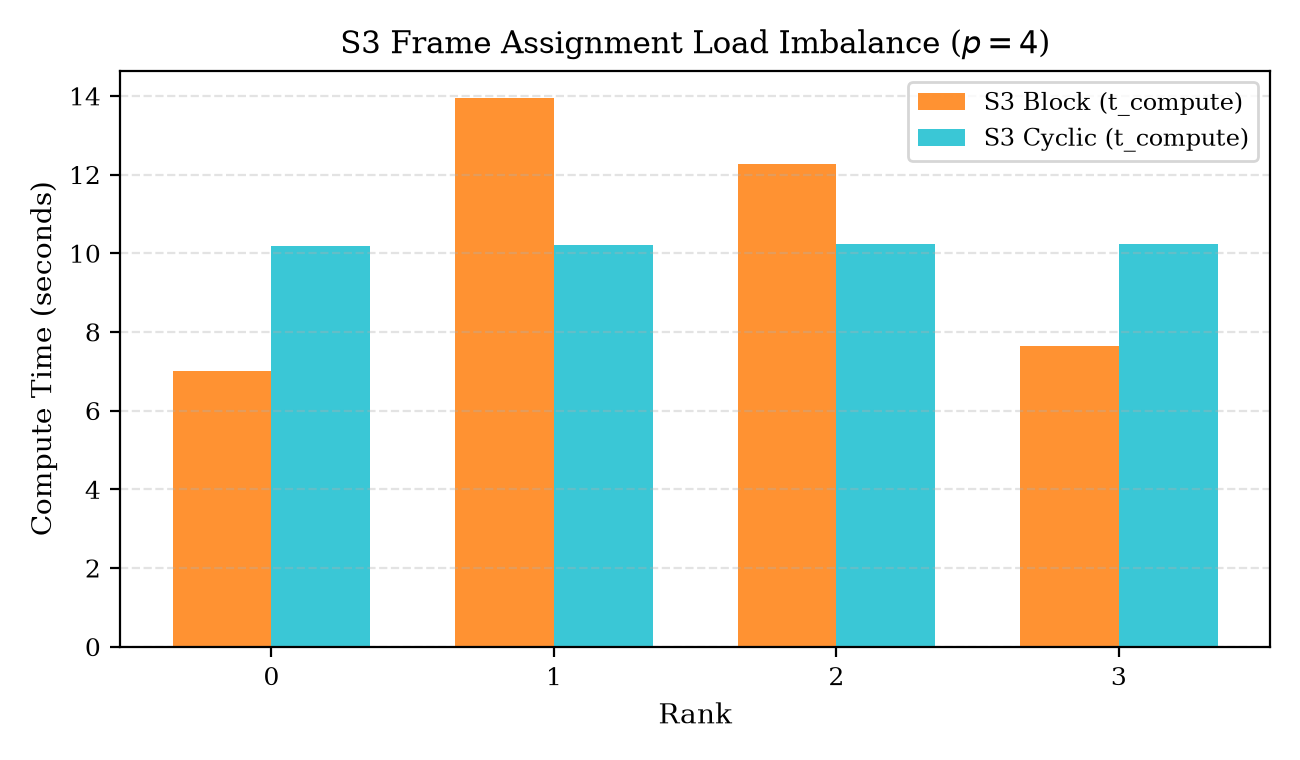
\includegraphics[width=0.60\linewidth]{fig6_s3_block_vs_cyclic.png}
\caption{S3 compute time per rank under Block vs. Cyclic assignment ($p=4$). Cyclic assignment interleaves cheap early frames with expensive deep frames across all ranks. Source: \texttt{results/busy\_time.csv}.}
\label{fig:s3_comp}
\end{figure}

\section{Iteration Count Cost Proxy Validation}
\label{app:cost}
Figure~\ref{fig:busy_vs_iter} validates that total iterations accurately predict measured CPU compute time across ranks.

\begin{figure}[htbp]
\centering
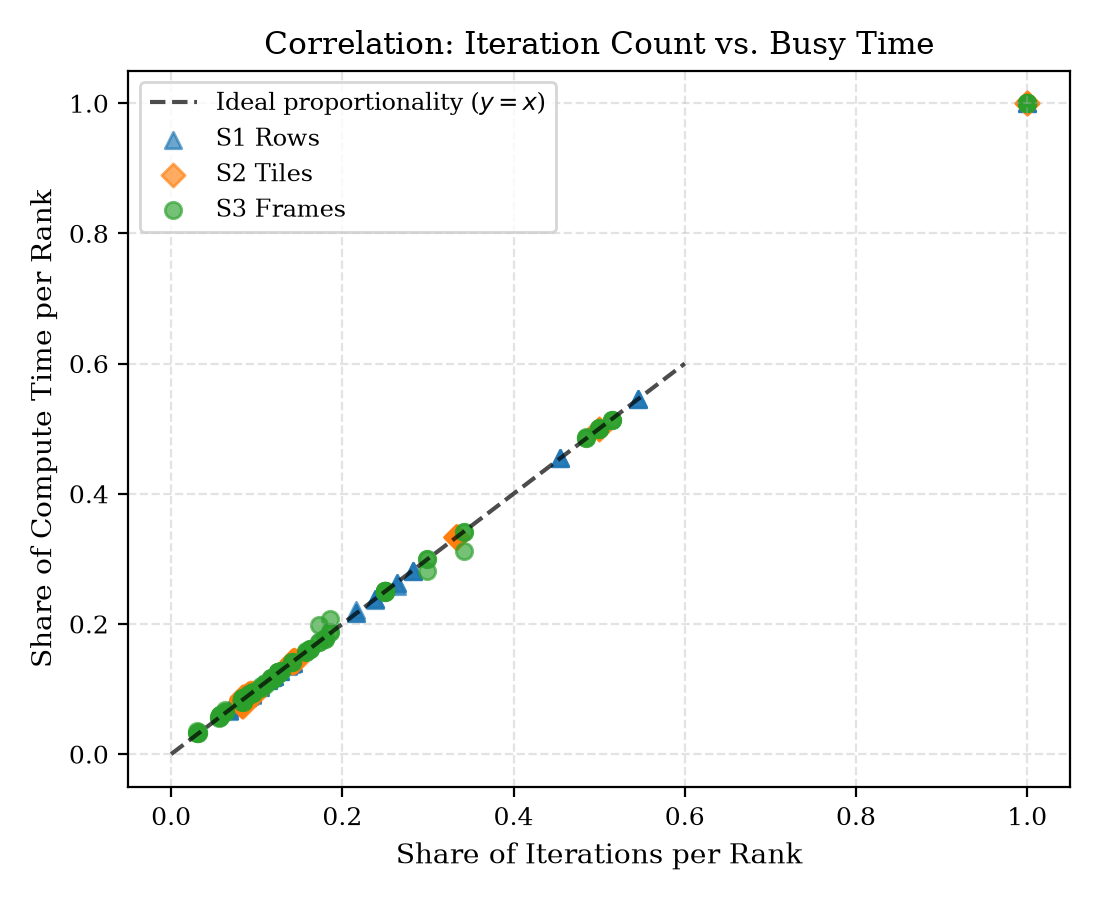
\includegraphics[width=0.52\linewidth]{fig5_busy_vs_iterations.png}
\caption{Correlation between rank share of total iterations and measured share of compute time. Source: \texttt{results/busy\_time.csv}.}
\label{fig:busy_vs_iter}
\end{figure}

\section{Local Shared-Memory Ping-Pong Communication}
\label{app:pingpong}
Table~\ref{tab:pingpong} and Figure~\ref{fig:pingpong} report the ping-pong latency and bandwidth curves across transfer buffer sizes.

\begin{table}[htbp]
\centering
\footnotesize
\setlength{\tabcolsep}{4pt}
\caption{MPI Ping-Pong latency and bandwidth on local shared memory. (Source: \texttt{results/pingpong.csv})}
\label{tab:pingpong}
\begin{tabular}{rcccc}
\toprule
\textbf{Message Size} & \textbf{Repetitions} & \textbf{Round-Trip} ($\mu$s) & \textbf{One-Way Latency} ($\mu$s) & \textbf{Bandwidth} (MB/s) \\
\midrule
1~B & 500 & 5.57 & 2.79 & 0.34 \\
8~B & 500 & 5.09 & 2.55 & 3.00 \\
64~B & 500 & 4.49 & 2.24 & 27.20 \\
512~B & 200 & 6.83 & 3.41 & 143.02 \\
4~KiB & 200 & 18.47 & 9.23 & 423.06 \\
32~KiB & 50 & 31.50 & 15.75 & 1984.00 \\
256~KiB & 50 & 149.08 & 74.54 & 3353.95 \\
1~MiB & 20 & 518.61 & 259.30 & 3856.46 \\
2~MiB & 20 & 1044.23 & 522.12 & 3830.57 \\
8~MiB & 10 & 4121.09 & 2060.55 & 3882.47 \\
\bottomrule
\end{tabular}
\end{table}


\begin{figure}[htbp]
\centering
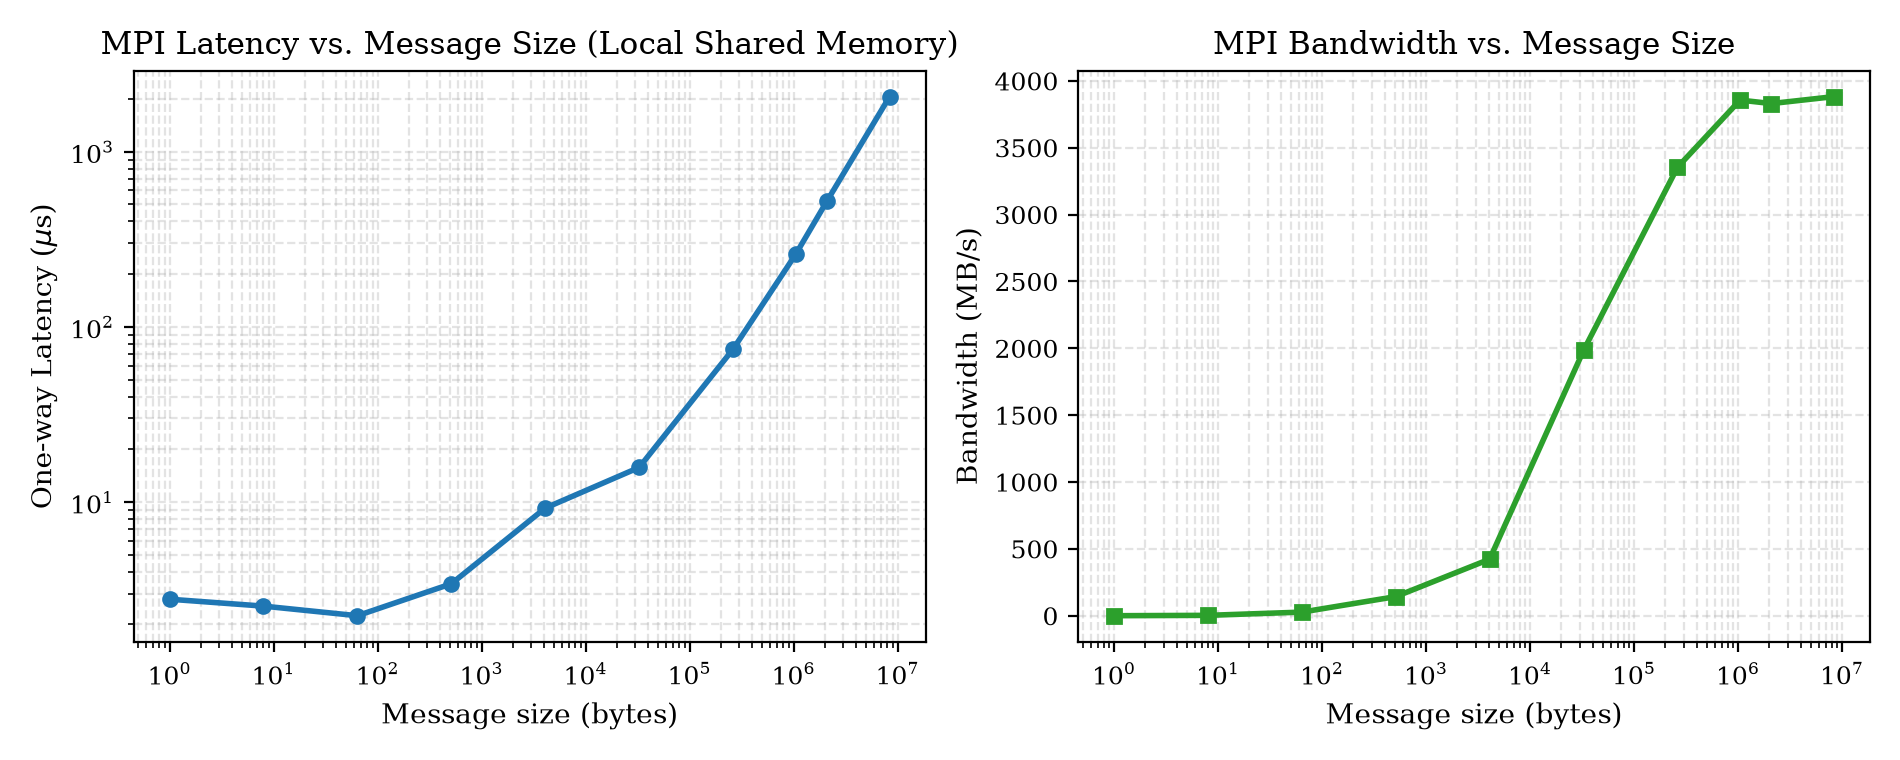
\includegraphics[width=0.82\linewidth]{fig7_pingpong.png}
\caption{Local MPI Ping-Pong latency (left) and bandwidth (right) vs. message size on host shared memory. Source: \texttt{results/pingpong.csv}.}
\label{fig:pingpong}
\end{figure}

\end{document}
